\documentclass[a4paper,11pt]{article}

\usepackage[utf8]{inputenc}
\usepackage{mathtools}
\usepackage[colorlinks=true, linkcolor=blue] {hyperref}
\usepackage{units}
\usepackage[english]{babel}
\usepackage{graphicx}
\usepackage[margin=1.25in]{geometry}


\pdfinfo{%
  /Title    (Probabilidad discreta)
  /Author   (Diego Ravignani)
  /Creator  ()
  /Producer ()
  /Subject  (Análisis estadístico de datos)
  /Keywords (Poisson, binomial, probabilidad)
}

\title{Probabilidad Discreta}
\author{Análisis Estadístico de Datos}
\date{}

\begin{document}
\maketitle

\begin{enumerate}

\item Dada la variable aleatoria $X$ y la constante $a$, calcular los siguientes valores en términos de $\mu=\mathrm{E}(X)$:

\begin{itemize}

    \item $\mathrm{E}(X+a)$

    \item $\mathrm{E}(a\,X)$
    
    \item $\mathrm{E}(X-\mu)$

    \item $\mathrm{E}( \mu \, X)$ 
    
\end{itemize}

\item Dada la variable aleatoria $X$ y la constante $a$, demostrar las siguientes identidades:

\begin{itemize}

    \item $\mathrm{Var}(X+a) = \mathrm{Var}(X)$
    
    \item $\mathrm{Var}(a\,X) = a^2 \, \mathrm{Var}(X)$

    \item $\mathrm{Var}(X) = \mathrm{E}(X^2) - \mathrm{E}(X)^2$
    
\end{itemize}

\item Dadas las variables independientes $X$ e $Y$, mostrar que:

\begin{itemize}

    \item $\mathrm{E}(X+Y) = \mathrm{E}(X) + \mathrm{E}(Y)$ 
    
    \item $\mathrm{Var}(X+Y) = \mathrm{Var}(X) + \mathrm{Var}(Y)$ 

\end{itemize}

\item Mostrar que la distribución binomial está normalizada a la unidad sumando todos los términos de la función de distribución de probabilidad.

\item \textbf{El test serológico de la covid-19.} Los tests serológicos detectan la presencia de anticuerpos en la sangre. \href{https://theconversation.com/coronavirus-tests-are-pretty-accurate-but-far-from-perfect-136671}{Este artículo} muestra una comparación de la sensitividad y especifidad de diez tipos de tests diferentes. Los investigadores encontraron que, como referencia, los tests son 90\% sensitivos y 95\% específicos. Suponiendo que solo el 10\% de la población tiene anticuerpos covid-19, calcular la probabilidad que una persona con un test positivo efectivamente tenga anticuerpos.

\item \textbf{Ayuda a Fermat.} La solución de Fermat al problema de la división justa de la bolsa es impráctica cuando quedan muchas rondas por jugar ya que implica contar todas las partidas que dan por ganador a uno de los dos jugadores. Afortunadamente con simulaciones Monte Carlo es posible encontrar una solución aproximada. Supongamos que un juego de 51 rondas es interrumpido en la ronda 25 y que Fermat ganó 15 rondas y Pascal 10. Simular el resto de las rondas para decidir cuál jugador gana la partida. Repetir este procedimiento 1000 veces para encontrar la división justa de la bolsa.
% fair.C

% \item Show that the mean of the sum of n Bernoulli variables with success probability $p$ is $\mu = n \, p$  and the variance is $\sigma^2 = n \, p \, (1-p)$. How can this help in the computation of the variance of a binomial variable?

% \item In general the mean of a function is different from the function evaluated at the mean ( $\mathrm{E}(f(X)) \ne f(\mathrm{E}(X))$. Show that this is the case for the binomial pdf with $f(X)=X^2$. 

% \item Simulate 100 throwings of a die and count how many times each number appears. Plot the resulting absolute and relative frequencies. Compare the relative frecuency with a uniform probability distribution function.
% dice.C

\item \textbf{El número de la suerte.} Simular el lanzamiento de cinco dados y contar cuántas veces sale el número tres. Repetir la operación 1000 veces y construir un histograma de frecuencia con el número de ocurrencias del número tres. Comparar los datos simulados con una función de distribución binomial con parámetros $n$ y $p$ adecuados. 
% binomial.C

\item \textbf{El jugador de dardos torpe.} Simular el lanzamiento de dardos considerando que el blanco interno de una diana estándar tiene un radio de \unit[12.7]{mm}, el blanco externo de \unit[31.8]{mm}, el anillo triple de \unit[107]{mm} y el anillo doble de \unit[170]{mm} como muestra la figura \ref{fig:dartboard}. Un jugador torpe lanza dardos al azar dentro del anillo doble de la diana. Calcular la probabilidad que un tiro individual dé en el blanco exterior. Simular una  corrida de 100 lanzamientos y contar cuántos dardos dan en el blanco exterior. Simular 1000 tandas de 100 lanzamientos y construir un histograma de frecuencia. Comparar con una distribución de Poisson.
% dart.C


%TODO Cambiar idioma de los labels con gimp 
\begin{figure} [htp]
\centering
\setlength{\abovecaptionskip}{0pt}
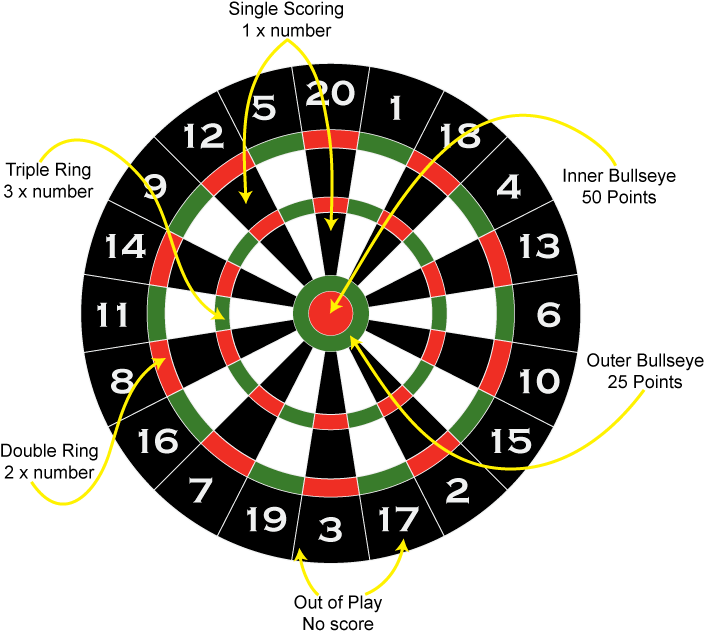
\includegraphics[width=.6\textwidth]{kindpng_1767452}
\caption{Diana de dardos estándar. \label{fig:dartboard}}
\end{figure}

%\item \textbf{(Para entregar)} Simular dos variables aleatorios $X_1$ y $X_2$ que siguen distribuciones de Poisson con parámetros $\mu_1=1$ y $\mu_2 = 2$ respectivamente. Calcular la variable $Y = X_1 + X_2$. Repetir la simulación 1000 veces. Graficar la distribución de la variable $Y$ y comparar con una distribución de probabilidad adecuada.
% poisum.C

% entregable 
%\item  Simular una variable aleatoria $Y$ que sigue una distribución de Poisson con parámetro $\mu = 10$. A continuación simular $Y$ variables de Bernoulli $X_i$ con $i = 1, ..., Y$ con parámetro $p=0.7$. Calcular el valor de una nueva variable $Z$ definida como $Z = \sum_{i=1}^Y X_i$. Repetir la simulación 1000 veces, construir un histograma de frecuencia de $Z$ y comparar con una distribución de Poisson. \emph{Nota: usar la distribución exacta sin ajustar los datos.}
% convo.C (ROOT), detector_ineficiente.ipynb (python)

% \item (optional) Show that the mean of a random variable $X$ following a binomial distribution of $N$ trials and success probability $p$ is $\mathrm{E}(X) = N p$.

% \item (optional) \href{https://international.ipums.org/international/}{IPUMS-International} is dedicated to collecting and distributing census data from around the world.  \href{https://drive.google.com/open?id=1kq6eLL9yj99keUGYOsXYpTkKZqc9s7gT}{This folder} contains an extract of 20 variables of 39158 persons (0.1\% sample) of the Argentina census of 2010. The folder includes the data extract (ipumsi\_00001.dat), the description of the data structure (ipums\_00001.cbk), and the description of the variables (ipums\_0001.xml). Write a program to read the ipums data extract and build a contingency table containing the sex of a person and whether she or he completed the secondary school. Check what codes of the variables EDATTAN and LEVELSCH correspond to this case. Is there any gender bias in the completion of secondary school? Repeat the exercise for people that at are least 20 years old.  

% \item Calcular momentos de la binomial???

% item Calcular momentos de Poisson???

\end{enumerate}

\end{document}
